\documentclass{../download/tPRS2e}

    \usepackage[english]{babel}
    \usepackage{tikz}
    \usetikzlibrary{patterns}
    \usepackage{graphicx}
    \graphicspath{{media/}}
    
\begin{document}

\title{On the Problem of Tool Air Move Minimization for Sheet Cutting CNC Machine}

\author{
\name{
Petunin A.A.\textsuperscript{a},
Polishuk E.G.\textsuperscript{a},
Ukolov S.S.\textsuperscript{a}$^{\ast}$\thanks{$^\ast$Corresponding author. Email: s.s.ukolov@urfu.ru}
}
\affil{
\textsuperscript{a}Ural Federal University, Yekaterinburg, Russia;
}}

\maketitle

\begin{abstract}
The problem of finding pierce points to get
minimal tool air move path length is considered
in case of standard cutting technique
(closed contours cutting).
Discrete approximation is discussed,
then a new algorigthm is described,
which perform no discretization,
ie. any point on a contour can be 
used for piercing operation.
\end{abstract}

\begin{keywords}
    contour;
    pierce point;
    minimal tool path;
\end{keywords}

During development of control programs for
CNC sheet cutting machines,
the problem of minimizing tool idle path
often appears.
One should select the order
of part contours to cut
and positions of pierce point on them,
so as total length of tool trajectory be minimal,
which implies,
that length of broken line connecting all
pierce points in the order of contour cutting
also be minimal.
In addition, a technological requierment should be met,
that if some contour lays inside another one,
the former must be processed before the latter.

Note, that we can consider
only contours containing no inner sub-contours.
Having got a solution for these contours,
one can easily add vertices
(pierce points) for the other contours,
preserving total length of the broken line.

\begin{enumerate}
    \item{}
To see this, let us denote by
$L_f$ the broken line length for original task
(for all contours considered)
and by 
$L_0$ that length for task with reduced set of contours.
Next we denote with $M$ and $N$
two vertices of the broken line for original task
($L_f$),
so as they belongs to remaining contours.
We can remove all intermediate links and connect 
$M$ to $N$ with line segment,
getting a new broken line with less or equal length.
So, $L_f \ge L_0$.
    \item{}
Let us consider broken line
having no vertex on some contour $C$.
One can find the \textbf{last} segment
of the broken line
that inersects $C$.
At least one such segment is known to exist,
because there is another contour inside $C$,
which in turn contains one vertex of the broken line.
The point of intersection $C \cup L_0$ can be inserted
into the broken line as new vertex,
giving a new broken line with the same length $L_0$
containg a vertex laying on the $C$.
Repeating this operation for all outer contours,
we get broken line $L_f$ with the same length
which conforms to above
technological constraint.
\end{enumerate}

Finally, $L_f = L_0$ and we can solve the problem,
considering only non-outer contours.

\begin{figure}[b]
    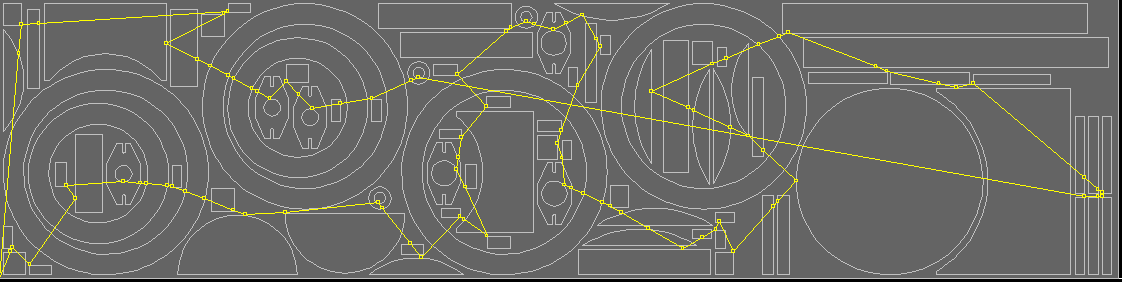
\includegraphics{mini-bad.png}
    \caption{Total length of path is 19649 mm}
\end{figure}

\begin{figure}[b]
    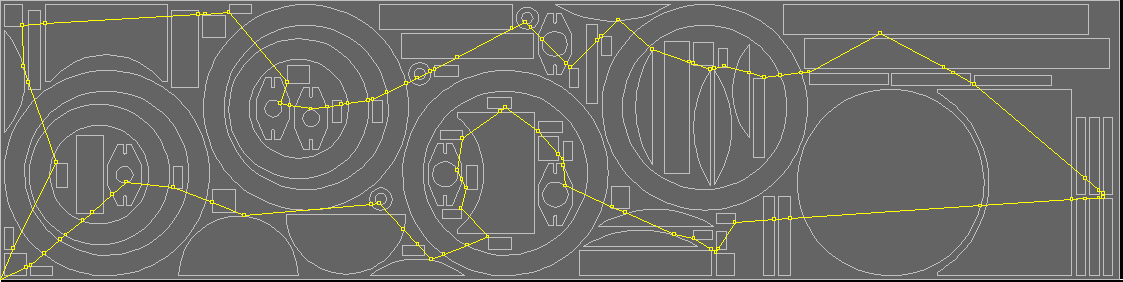
\includegraphics{mini-good.png}
    \caption{Total length of path is 15836 mm}
\end{figure}

\end{document}
